Vagueness and context-dependence of gradable adjectives have been promisingly formalized in computational models within the Rational Speech Act framework ---  a suite of game-theoretically oriented recursive models of pragmatic language understanding \parencite[e.g.,][]{goodman2016, lassiter2017adjectival, tessler2017warm}. Introduced by \textcite{frank2012predicting}, the Rational Speech Act framework is well in line with recent insights in Bayesian cognitive modelling, showing a great deal of flexibility to account for various phenomena studied in pragmatics like scalar implicature, hyperbolic language or generics, among many others \parencite[e.g.,][]{tenenbaum2011grow, problang}. This chapter reviews the basics of Rational Speech Act models and specifically prior models of gradable adjectives. While accounting for many aspects of gradable adjectives, many of those models assumed an a priori fixed comparison class. Yet as shown empirically in the previous Chapter \ref{chapter04}, listeners flexibly reason about the intended comparison class by taking into account syntactic and contextual cues. Therefore, this chapter attempts to propose a minimal extension to existing RSA-models which will formalize the reference-predication trade-off hypothesis of comparison class inference.%, allowing to flexibly incorporate reasoning about context and role of the noun in comparison class inference. 
  
\section{Understanding Rational Speech Act Models}
\label{intro-rsa}
Language is fascinatingly flexible and efficient, and largely so because interlocutors do not have to explicitly encode all information in utterances they produce, but instead rely on each other's ability to infer many aspects of the message from linguistic and situational context. In particular, pragmatic models of communication posit that given these contextual constrains, speakers and listeners can efficiently \emph{reason about each other's intended meaning of utterances} under one important assumption: speakers are approximately \emph{rational} with respect to their communicative goals \parencite{frank2012predicting}. The Rational Speech Act framework (henceforth: RSA) views this process of establishing the intended meaning as recursive reasoning between speaker and listener: in interpretation-oriented models, a pragmatic listener $L_1$ infers a state of the world intended to be conveyed by a rational speaker $S_1$, by using \emph{Bayesian inference} to reason about likely world states given the observed utterance, given that the speaker $S_1$ chooses utterances according to their most likely semantic interpretation by a literal listener $L_0$ \parencite{problang}.  

The idea of language as rational action produced by \emph{cooperative} interlocutors was formulated by \textcite{grice1975logic}. The core of his proposal are four conversational maxims that speakers are thought to stick to when producing utterances in order to convey particular messages: the \emph{maxims of relation} (contributions made to the conversation should be relevant), \emph{quantity} (the contributions should be as informative as required, but not more so), \emph{quality} (the speaker is supposed to believe their contributions to be true) and \emph{manner} (the way the contributions are expressed should be perspicuous). Listeners then reason about intended messages in light of these maxims \parencite{grice1975logic}.

Grice’s ideas became particularly influential when precise information-theoretic formalisations of such vague concepts like \emph{informativeness, cooperation} and \emph{relevance} were proposed, and, informed by insights from game-theory, gave rise to RSA \parencite{frank2012predicting}.
In particular, RSA captures cooperative coordination of intended meaning between interlocutors via recursive application of probabilistic mechanisms; and relevance or informativeness of utterances is captured as the \emph{utility} of the utterance in helping the listener reduce uncertainty in their beliefs about the world, where these beliefs can be represented as a probability distribution over possible states of the world \parencite[as advocated by e.g.][]{tenenbaum2011grow}.  
That is, listeners update their beliefs about the world via Bayes' rule upon hearing an utterance produced by an informative speaker \parencite{frank2012predicting}.\footnote{Familiarity with basic notions in probability and Bayesian inference is presupposed here. For a review of aspects relevant for RSA, \textcite[see e.g.][]{lassiter2017adjectival}.}

The mechanisms of RSA are best illustrated by a simple example from a reference game, described by \textcite{frank2012predicting}.
Consider a simple world consisting of a context $C$ = \{blue square, blue circle, green square\} (Fig. \ref{rsa-scene}).
\begin{figure*}[t]
	\begin{center}
		
\includegraphics[width=0.5\linewidth]{rsa_scene.png}
	\end{center}
	\vspace{-0.3cm}
	\caption{A simple reference resolution example scenario: the context $C$ consists of three possible referents \parencite{frank2012predicting}}
	\label{rsa-scene}
\end{figure*}
In a reference game scenario, a speaker wants to communicate to a listener a particular referent $s$ in context $C$, e.g., the blue square. To do so, she has a finite set of utterances $U = \{blue, green, square, circle\}$.\footnote{The finite fixed set of alternative utterances is a crucial assumption made in RSA. It is an important question for future research how interlocutors actually determine this set of relevant alternatives.} A listener then tries to recover the intended referent (i.e., the blue square) upon receiving an utterance (e.g., ``blue"). 
As mentioned above, standard RSA models consist of three layers: a pragmatic speaker $S_1$ who chooses an optimal utterance for signalling $s$ (the blue square) to a literal listener $L_0$, who infers all the referents consistent with the literal meaning of the utterance $u$ ('blue'), and a pragmatic listener $L_1$ who reasons about this speaker behaviour given a particular utterance $u$ ('blue'), using Bayes' rule.

So the basis of RSA models is the na\"ive literal listener agent $L_0$ that $S_1$ reasons about when choosing an optimal utterance to communicate the blue square, who computes a probability distribution over possible referents in context $C$  consistent with the received utterance $u$: %\pt{function that maps each utterance to the probability distribution over world states}
\begin{equation}
P_{L_0}(s \mid u, C) = \frac{\llbracket u \rrbracket (s) \; P(s)}{\sum_{s' \in C} \llbracket u \rrbracket (s') \; P(s')}
\end{equation}
The context $C$ is typically assumed to be shared between speaker and listener, so it will be dropped in further derivations for simplicity. Given that the denominator is a constant, it can also be dropped for simplicity, so that the probability of a particular state $s$ given utterance $u$ is proportional to the literal meaning $\llbracket u \rrbracket (s)$ and the prior probability of $s$: 
\begin{equation}
P_{L_0}(s \mid u) \propto \llbracket u \rrbracket (s) \; P(s)
\end{equation}
The prior $P(s)$ is the prior belief of $L_0$ about which states are likely to be communicated by the speaker. Typically, a uniform prior is used, indicating that a priori any state is as likely as others, but relevant contextual information like perceptual salience or frequency of some referents might be encoded in this prior \parencite{frank2012predicting}.

The second component of the $L_0$ is the \emph{literal meaning} of the observed utterance $u$ (indicated as $\llbracket u \rrbracket$). In RSA, literal semantics computation is based on a form of Montague’s compositional semantics, typically assuming a mapping from particular states to Boolean truth-values \parencite{montague1973proper} \parencite[but see e.g.][for alternative approaches]{degen2020redundancy}. 
So, for instance for the context in Fig. \ref{rsa-scene}, applying the utterance `circle' to the blue square would return \texttt{false}, but `blue' would return \texttt{true}:
\begin{align}
\llbracket circle \rrbracket (blue \: square) = 0 \notag \\
\llbracket blue \rrbracket (blue\: square) = 1
\end{align}
  
So for our example utterance `blue' the literal listener $L_0$ infers a uniform distribution over the blue circle and the blue square, since the utterance equally applies to both objects (Table \ref{rsa-l0}):

\begin{table}[h]
	\begin{center}
		\caption{The probability distribution over states inferred by $L_0$ when hearing the utterance `blue' in context $C$.}
		\label{rsa-l0}
		\vskip 0.12in
		\begin{tabular}{cc}
			State & Probability \\
			\hline
			blue circle & 0.5 \\
			blue square & 0.5 \\
			\hline
		\end{tabular}
	\end{center}
\end{table}

The next RSA layer is the pragmatic speaker $S_1$. $S_1$ is modelled as an agent who chooses an utterance $u$ rationally, i.e., according to its expected utility, in order to communicate a particular state of the world $s$ in context $C$ to $L_0$. This is captured in the speaker-utility function $U_{S_1}(u; s)$, which trades-off the informativity of an utterance for $L_0$ with non-negative cost $C(u)$ of producing the particular utterance \parencite{problang}:
\begin{equation}
U_{S_1} (u;s) = log L_0(s \mid u) - C(u)
\end{equation}
In information-theoretic terms, $L_0$ provides a hook within this utility function to compute the \emph{informativeness} of particular utterances as communicating particular states, 
where informativeness is quantified by surprisal --- a measure of how much uttering a particular $u$ reduces uncertainty about the state of the world, given that $u$ is \emph{true of $s$} (i.e., $\llbracket u \rrbracket (s) = 1$) \parencite{frank2012predicting}: 
\begin{equation}
I_{ \tilde{u} (s)}(s) = -log(\tilde{u} (s))
\end{equation}
$I_{\tilde{u} (s)}(s)$ measures how much information $L_0$ gains when hearing the utterance $u$, assuming a known distribution $\tilde{u} (s)$ over states that are coveyed by the literal interpretation $\llbracket u \rrbracket$ which implies the probability of $s$; i.e., it measures how \emph{surprising} it would be to observe $s$ having observed $u$.
Intuitively, assuming a uniform $\tilde{u} (s)$, the less states an utterance applies to, the lower is the surprisal of a particular state, and the higher is its informativeness. Here, informativeness is used in a relatively informal way, meaning that a maximally informative utterance conveys a message maximally unambiguously. For instance, in the context of Fig.~\ref{rsa-scene}, the utterance `circle' is highly informative, because there is only one object it applies to, while the utterance `blue' is less informative because it applies to two objects. 
Therefore, the speaker utility is anti-proportional to the surprisal of the utterance \parencite{frank2012predicting}:
\begin{equation}
U_{S_1} (u;s) = -(-log(\tilde{u}(s))) - C(u) = log L_0(s \mid u) - C(u)
\end{equation}
%: speakers strive to choose an utterance minimizing surprisal of a particular state of the world given that utterance. 
The cost function $C(u)$ is also an important tool for integrating psychologically plausible information about speaker-biases, like frequency or phonological complexity of producing particular utterances compared to others. Now the rational speaker $S_1$ maximizes the probability of conveying the intended state of the world $s$ acting according to Bayesian decision theory, by choosing an utterance $u$ proportionally to its expected utility described by the \emph{softmax} function:
\begin{equation}
P_{S_1}(u \mid s) = \frac{e^{\alpha \: U_{S_1} (u; s)}}{\sum_{u' \in U s.t. u'(s) = true} e^{\alpha \: U_{S_1} (u'; s)}}
\end{equation}
The parameter $\alpha$ controls the speaker's \emph{optimality}, assuming $\alpha = 1$ in examples used here; for $\alpha = \infty $ the fully rational decision rule used in game-theory can be recovered \parencite{problang, lassiter2017adjectival}.

For this example, $S_1$ chooses an utterance $u$ maximizing the probability of the state `blue square' being recovered by $L_0$. So $S_1$ infers a distribution over utterances applicable to the target `blue square' (Table \ref{rsa-s1}):

\begin{table}[h]
	\begin{center}
		\caption{The probability distribution over utterance inferred by the pragmatic speaker $S_1$ in order to communicate the referent `blue square'}
		\label{rsa-s1}
		\vskip 0.12in
		\begin{tabular}{cc}
			Utterance & Probability \\
			\hline
			blue & 0.5 \\
			square & 0.5
		\end{tabular}
	\end{center}
\end{table}
 
Finally the top-level layer, the pragmatic listener $L_1$, reasons about this utterance-generating speaker behaviour given a particular utterance $u$ (`blue'), using Bayes' rule:\footnote{This recursive depth of three model layers is a common assumption in RSA models, and requires a reasonable amount of computational resources \parencite{lassiter2017adjectival}. Yet this is just a practical approximation, and some models (e.g., production-oriented models) employ additional levels \parencite{problang}.}
\begin{equation}
\label{vanilla-l1} 
P_{L_1}(s \mid u) = \frac{P_{S_1}(u \mid s) \; P(s)}{\sum_{s' \in C} P_{S_1}(u \mid s') \; P(s')}
\end{equation}
That is, the probability of a particular state $s$ (i.e., blue square) given the utterance $u$ (`blue') is equal to the probability that the pragmatic speaker $S_1$ would choose `blue' in order to convey the \textit{blue square}, multiplied by the prior probability $P(s)$ of occurence of state $s = blue \:square$, normalised by a constant sum of probabilities of all possible speaker behaviors for all possible states $s'$. 
Equation \ref{vanilla-l1} shows that the posterior over states $s$ given an utterance $u$ is proportional to the speaker production probability $P_{S_1}(u \mid s)$ times the state prior $P(s)$ because the denominator is a constant: 
\begin{equation}
P_{L_1}(s \mid u) \propto P_{S_1}(u \mid s) \; P(s)
\end{equation} 
Interestingly, the state prior $P(s)$ might differ between $L_0$ and $L_1$, e.g., incorporating prior world knowledge of the pragmatic agent $L_1$, but being uniform for the na\"ive agent $L_0$ \parencite{problang}. 

In this example, upon hearing `blue', $L_1$ infers that the speaker is more likely to convey the blue square (Table \ref{rsa-l1}):

\begin{table}[h]
	\begin{center}
		\caption{The probability distribution over referents inferred by the pragmatic listener $L_1$ upon hearing the utterance `blue'.}
		\label{rsa-l1}
		\vskip 0.12in
		\begin{tabular}{cc}
			State & Probability \\
			\hline
			blue square & 0.6 \\
			blue circle & 0.4
		\end{tabular}
	\end{center}
\end{table}
\begin{figure*}[t]
	\begin{center}
		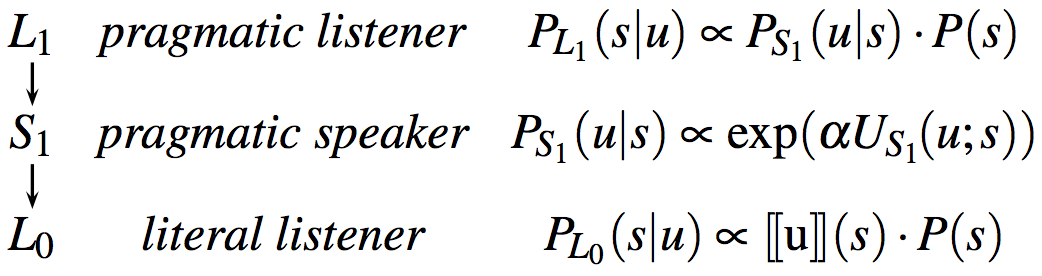
\includegraphics[width=0.5\linewidth]{vanilla-rsa.png}
	\end{center}
	\vspace{-0.3cm}
	\caption{A schematic depiction of a vanilla RSA model \parencite{problang}.}
	\label{vanilla-rsa}
\end{figure*}
Putting all the elements together results in the vanilla version of an RSA-model (Fig.~\ref{vanilla-rsa}).
The crucial illustration of the RSA mechanism is the difference between the distributions inferred by $L_0$ and $L_1$ upon observing the same utterance `blue'. Reasoning about the utterance-generating speaker-model incorporated in $L_1$, while $L_0$ acts according to literal semantics only, is crucial for the pattern of interpretation we observe: $L_1$ infers that the speaker is more likely to mean the blue square, because if she had meant the blue circle, she could have said `circle', which would have been less ambiguous, and therefore more informative (Table \ref{rsa-l1}). That is, $L_1$ does not only consider what the speaker actually said, but also what the speaker \emph{could have said}. In contrast, $L_0$ infers equal probabilities of `blue' meaning `blue square' or `blue circle' because the utterance is literally true of both referents (Table \ref{rsa-l0}). Crucially, this pattern predicted by the RSA-model is well in line with rational behaviour of humans gathered empirically in such reference game scenarios, confirming that human interlocutors make use of more than just the literal semantics of their words when communicating \parencite{frank2012predicting, problang}.

%Having set the basic building blocks of RSA models, some more sophisticated features of RSA relevant for modelling adjectives should be mentioned. 

%note that these exist as part of L1's reasoning \parencite{lassiter2017adjectival}
\section{Previous RSA Models of Gradable Adjectives}
In this section, previous RSA models of gradable adjectives are discussed; they showed that RSA is a flexible tool suitable to integrate more complex pragmatic reasoning required for interpreting vague expressions.
%threshold semantics, where the threshold is probabilistically inferred \parencite{lassiter2017adjectival} for a given comparison class.

\textcite{lassiter2013context} first provided a model of gradable adjective interpretation within the RSA-framework, showing that pragmatic reasoning can capture their meaning via inference over the latent standard of comparison variable $\theta$ underlying the vague semantics (s. Chapter \ref{chapter02}). %Importantly, probabilistic reasoning provides tools to capture uncertainty over certain aspects of the message, in this particular case - the speaker’s intended meaning of the adjectival utterance.  
The proposed model builds upon the standard RSA model with three levels, adding one crucial extension: the pragmatic listener $L_1$ jointly infers the value of the threshold $\theta$ along with the state of the world $s$ (i.e., the degree to which a referent possesses the property described by the adjective):
\begin{equation}
P_{L_1} (s, \theta \mid u) \propto P_{S_1} (u \mid s, \theta) \; P (s) \; P(\theta)
\end{equation} 

The model formalized literal meaning of gradable adjectives in terms of degree-semantics, assuming that the lexical entry of the adjective specifies the underlying scale and its polarity (cf. Chapter~\ref{chapter02}):
\begin{equation}
\llbracket u \rrbracket^{\theta} (s) = s > \theta
\end{equation}
However, the literal meaning of the adjective by itself is underspecified --- it depends on the pragmatically recovered threshold $\theta$, which in turn depends on the comparison class used in the particular context; yet, like vanilla RSA the model is anchored in the literal interpretation of the adjective applied to a referent at the level of $L_0$.  
So in order to allow specifying the $L_0$ which requires computing the truth-value of an utterance for a given state, the authors proposed $L_1$ consider all possible assignments of the \emph{lifted} latent variable value $\theta$, given a prior over that variable $P(\theta)$. A uniform $P(\theta)$ encoded that a priori any property degree might qualify for being described by the adjective. Crucially, the state prior $P(s)$ encoded prior knowledge about \emph{likely property degrees for a specific comparison class} which the referent might have. For instance, the difference in the meanings of \emph{big} in `big for a tree' and `big for a pug' would be encoded in different priors over the likely properties of the respective referents. It is common practice to quantify this prior knowledge empirically via prior elicitation experiments \parencite{problang}.

The assumed $\theta$ values are then iteratively passed down through the model. Given a particular value, the speaker-model can be specified:
\begin{equation}
	P_{S_1} (u \mid s, \theta) \propto exp(\alpha \: log (P_{L_0} (s \mid u, \theta) - C(u)) )
\end{equation}	

Then, in contrast to $L_1$ who is uncertain about $\theta$, $L_0$ interprets the utterance literally, so she gets $\theta$ passed down and infers the state distribution consistent with this particular $\theta$ assignment and the observed adjective $u$:
\begin{equation}
P_{L_0} (s \mid u, \theta) = P_{L_0} (s \mid \llbracket u \rrbracket ^\theta = 1 ) \propto \llbracket u \rrbracket ^\theta (s) \; P(s)
\end{equation}

So putting all the layers together, $L_1$ can compute a joint posterior distribution over all possible combinations of states and values of the latent threshold $\theta$ lifted to the level of the pragmatic listener. Notably, \textcite{lassiter2013context} assumed the relevant comparison class to be supplied to the listener, such that she was uncertain only about the standard of comparison. Yet as discussed in chapters \ref{chapter02}-\ref{chapter03} and shown empirically in Chapter \ref{chapter04}, listeners flexibly reason about the intended comparison class because there might be multiple a priori plausible options in absence of an explicit \emph{for}-phrase.

\textcite{tessler2017warm} introduced an RSA-model of gradable adjectives accounting for flexible reasoning about the relevant comparison class via world knowledge (the rationale and behavioural experiments of this study are described in detail in Section~\ref{2.4.}). In particular, in the proposed model the listener is not only uncertain about the standard of comparison $\theta$, but also about the specificity of the relevant comparison class $c$ (superordinate~vs.~subordinate category of the referent), given prior knowledge about typical property distributions in each category. %That is, listeners were assumed to know the a priori probability that an adjective could felicitously apply to a referent given its category, assuming a specific comparison class; 
They used this knowledge to infer the intended comparison class upon hearing a simple adjectival utterance $u$ of the form `\emph{PRON} is \emph{ADJ}' said of a referent whose \emph{subordinate category was known to the listener}.
Similarly to the model proposed by \textcite{lassiter2013context}, the pragmatic listener iterated over all possible value assignments of the lifted $\theta$ variable when reasoning about the utterance-generating process, to jointly infer the property degree $s$, the threshold $\theta$ and the relevant comparison class $c$, given the utterance $u$:
\begin{equation}
P_{L_1}(s, \theta, c \mid u) \propto P_{S_1} ( u \mid s, \theta, c) \; P(s \mid c_{sub}) \; P(c) \; P(\theta)
\end{equation} 
That is, the listener reasoned about how a rational speaker $P_{S_1}$ would behave in order to communicate a specific property, given a comparison class and a threshold, together with their prior knowledge about what property degrees are plausible given the subordinate category $P(s \mid c _{sub})$ the referent belongs to, and their prior beliefs $P(c)$ about which comparison class categories are likely to be used and what properties are likely to qualify for applying the adjective ($P(\theta)$). Accordingly, the speaker-model $P_{S_1}( u \mid s, \theta, c)$ can be specified assuming particular values of the property, the comparison class and the threshold:
\begin{equation}
P_{S_1}( u \mid s, \theta, c) \propto exp(\alpha \: log P_{L_0} (s \mid u, \theta, c))
\end{equation}

The $L_0$ again specified a literal listener who interpreted the adjective $u$ according to its literal semantics, assuming a particular comparison class $c$ and $\theta$:
\begin{equation}
P_{L_0}(s \mid u, \theta, c) \propto \llbracket u \rrbracket_{\theta} (s) \; P( s \mid c)
\end{equation}  
Importantly, $L_0$ sampled states according to a prior $P(s|c)$ specified by the received comparison class $c$, which integrated the comparison class into the literal semantics of the adjective. 

Since the predictions of this model strongly depend on prior world knowledge, it is important how the property priors given different comparison classes were specified. \textcite{tessler2017warm} fixed superordinate property distributions as $\mathcal{N} (0, 1)$ and subordinate property distributions as $\mathcal{N}(\mu_{sub}, \sigma_{sub})$, inferring the paramters of subordinate distributions from experimental data. The comparison class prior $P(c)$ was approxiamted via empirical Google WebGram frequencies of usage of the respective comparison class labels. 

\textcite{tessler2017warm} showed that the model captures human inferences discussed in Section \ref{2.4.} very well, confirming the role of world knowledge for comparison class inference. 
% potential spot to integrate Dan Yurovsky's work 
However, this model only considered the effect of world knowledge on comparison class inference, and focused on interpretation of simple underspecified utterances of the form 'He is tall'. In the following section, a further extension of previous RSA models is proposed, which accounts for more complex sentences containing a noun and integrates more sophisticated reasoning about several aspects contributing to comparison class inference.  

\section{Reference and Predication in RSA}
This section outlines a novel RSA model formalizing the reference-predication trade-off hypothesis.

First, let's recall the reference-predication trade-off hypothesis: it posits that speakers pursue particular \emph{informational goals --- reference} and \emph{predication} --- when crafting their utterances. These informational goals are realized by the speaker syntactically via different positions of the noun: the noun is more likely to contribute to reference when appearing in the sentence subject, especially when combining with the deictic ``that", but less likely to do so when appearing in the predicate. Listeners, in turn, reason about these speaker goals when interpreting the observed utterance.  Hence, nouns appearing in the subject can be potentially \emph{explained away} by their utility in reference, while nouns appearing in the predicate  are less likely to contribute to reference and therefore more likely to contribute to predication --- i.e., constrain the comparison class. 
Therefore, the degree to which the noun of the sentence constrains the comparison class --- i.e., serves predication --- trades off with its utility in reference. 

\subsection{Questions Under Discussion in RSA}
\label{rsa-qud}
Reasoning about particular informational, or conversational, goals is closely related to basic assumptions made in RSA.
As described in Section~\ref{intro-rsa}, the speaker is assumed to be a rational agent producing utterances of optimal utility with respect to some specific \emph{conversational goal} determined by discourse, also called \emph{question under discussion (QUD)}  \parencite{lassiter2017adjectival, roberts2012information}. The communication is structured so as to maximize the probability that the listener infers the intended \emph{answer to this QUD}. In the vanilla example introduced in Section~\ref{intro-rsa}, the QUD was to determine the referent, and the answer intended by the speaker was `blue square'. From this perspective, interlocutors' contributions to discourse are \emph{relevant} if and only if they contribute to answering the question under discussion \parencite{roberts2012information}. Note that such questions under discussions might indeed be realized by specific speech acts, but do not have to be --- they often remain implicit, and resemble questions rather formally in that they proffer the set of relevant alternatives interlocutors commit to addressing. Yet, interlocutors are fascinatingly good at determining the QUD pragmatically so as to functionally organize their communication around the QUD; they might do so by using different strategies, one prominent strategy in English being to make use of focus \parencite{roberts2012information, krifka2008basic}. But they might also employ other strategies, like choosing particular syntactic structures over others --- e.g., as proposed by the reference-predication trade-off hypothesis.  

From a semantic perspective, utterances then might have several dimensions of interpretation, each dimension corresponding to the interpretation of the utterance satisfying a distinct communicative goal, or answering a distinct QUD. This idea was first formlazed within the RSA-framework by \textcite{kao2014nonliteral}, applied to hyperbolic and pragmatic halo effects in interpretation of number words. The crucial novelty they introduced was listener uncertainty about the relevant QUD along with the multi-dimensional literal meaning of utterances, where each dimension satisfied a distinct potential QUD. The speaker in this model chose utterances optimally conveying her particular intended QUD \parencite{kao2014nonliteral}. %\pt{add formulas if necessary}

Another approach to formalizing multiple conversational goals was taken by \textcite{yoon2016talking} who proposed a model of polite language. The authors noted that although politeness phenomena were argued to violate basic cooperative principles of quality, they can be explained as produced by rational interlocutors pursuing not only the goal of informativeness, but simultaneously also a \emph{social goal} \parencite[cf.][]{brown1987politeness, yoon2016talking}. That is, by using polite sentences speakers strive to trade off being informative and saving the listener's self-image, or \emph{face}. Omitting here the details of how exactly this social goal was formalized, the authors proposed a model wherein the speaker tried to balance the utility of an utterance as simulatneously achieving the social goal and the goal of being maximally informative. She did so by maximizing a global utility function, which consisted of a weighted combination of these two utility sub-functions. The pragmatic listener then reasoned about the exact weighting of these two goals \parencite{yoon2016talking}. 

Yet the majority of RSA models usually assume that speakers address one particular conversational goal. The listener might be uncertain about it, as in case of QUD-models, but mostly models might just addressed one pre-defined aspect of communication, i.e., one QUD \parencite[see][for an overview of various RSA models]{problang}. 

This work has argued that interlocutors at least consider multiple informational goals (i.e., QUDs) that might be addressed within the same utterance containing a noun and a gradable adjective, reasoning how different parts of the utterance might probabilistically contribute to achieving each of the goals. Therefore, in the following a model is proposed which attempts to formalize the reference-predication hypothesis. It treats speakers' choice of utterances as \emph{incremental}, where the subject is chosen so as to establish reference, and the predicate is chosen to convey the comparison class --- and so one utterance is optimized to fulfil multiple QUDs. 

\subsection{Refpred-RSA Model}
\label{refpred-rsa}
In the following, the basic structure of the novel reference-predication RSA-model is presented. %Then, different potential representations of the speaker-utility function integrated in that basic structure are presented and discussed.
Then, model predictions are qualitatively compared to the results of the Comparison Class Inference Experiment (s.~Section~\ref{experiment3}). It will be shown that minimal extensions to existing models result in accurate predictions about the identity of an unknown referent, its property, and crucially, the intended comparison class. 
%It will be shown that minimal extensions to existing models result in accurate predictions about identity of an unknown referent and its property, but predictions about the lifted comparison-class variables are limited if assuming the representation used by \textcite{tessler2017warm}. 
The model is intended to predict comparsion class inferences drawn from sentences differing in the type of the noun (basic~vs.~subordinate referent label) and its position (subject~vs.~predicate) used in different contexts (basic~vs.~subordinate), investigated empirically in Experiment 3 (s.~Section~\ref{experiment3}). The anaphoric ``one" condition is disregared, because it was rather an experimental sanity-check condition. This model is inspired by previous gradable adjective interpretation models: The meaning of adjectives is represented in terms of threshold semantics, similarly to the proposal by \textcite{lassiter2013context}; the comparison class representation is inspired by the model by \textcite{tessler2017warm}.

In the model, upon hearing an utterance of the form ``That N is ADJ" or ``That's a ADJ N" the pragmatic listener tries to resolve his uncertainty about the specific member of the context the speaker is referring to, its size and the comparison class intended by the speaker. As a first approximation, driven by present experimental results and previous work by \textcite{tessler2017warm}, it is assumed that the potential comparison class is either the subordinate or the basic-level category of that referent. The potential referent might be one of the members of the perceptual context (i.e., basic-level or subordinate context), though the listener knows the subordinate category of the intended referent ($r\_{sub}$).\footnote{Note that this representation might not fully correspond to experimental set-up: The intended referents of the sentences were made salient by presenting them in a picture separate from the context. However, if anything, this representation might be seen as more conservative than the empirical set-up, because it generally puts a higher referential pressure on the speaker.} Therefore, the listener is assumed to have access to the subordinate categories of all possible referents, which inform their potential sizes.
Formally, the listener infers the comparison class $cc$, the referent $r$ and its size $s$ given an utterance $u$ and a perceptual context $C$:
\begin{equation}
P_{L_1} (r, s, cc \mid u, C) \propto P_{S_1} (u, cc \mid s, r, C) \; P(r, s \mid C, cc_{r\_sub}) 
\end{equation}
That is, the listener infers the referent, its size and the comparison class by reasoning about how a speaker would behave in order to communicate a particular referent and its size in context, in addition to his prior knowledge about properties of different subordinate categories. All referents in context consistent with the subordinate category of the intended target are treated as equally likely to be discussed, but more sophisticated models might upgrade the prior to incorporate perceptual salience, for instance based on the size of referents. 

Importantly, rather than representing the comparison class as a variable lifted to the level of the pragamtic listener $L_1$ \parencite[as proposed by][]{tessler2017warm}, the intended comparison class influencing the resolution of the adjective is represented as a concious \emph{lexical choice, or a local enrichment} made by the speaker \parencite[e.g., discussed for other phenomena by][]{chierchia2012grammatical, problang}. So while the pragmatic listener in \textcite{tessler2017warm} assumes that the speaker has a fixed meaning of the adjective (e.g., ``big for a dog" or ``big for a Great Dane") which the listener is uncertain about, in the current model the pragmatic listener reasons about a speaker who might \emph{variably} choose her intended adjective meaning \parencite[cf.][]{problang}. 
This was proposed in prior work arguing that pragmatic enrichments might already take place at subsentential --- i.e., lexical --- level, such that the speaker chooses to convey one of grammatically supplied local phrase readings with her utterance \parencite[for instance, applied to scalar implicatures by][]{chierchia2012grammatical}. In the current case, the speaker can choose between the subordinate and basic-level comparison class relative to which the adjective will be interpreted, in addition to the option to use a predicative noun as the comparison class. 
%\pt{add some explanations/background on what local enrichment is from Chierchia } 

So the speaker determines an \emph{optimal utterance and comparison class} in order to communicate a referent and its size, given the adjective she wants to use and the context, by optimizing the speaker-utility function $U$:
\begin{equation}
P_{S_1} (u, cc \mid s, r, C)  \propto exp(\alpha \: U_{S_1}(u; s; r; cc; C) \; P(cc) \; P(u)) 
\end{equation}
The cost of producing uterances $C(u)$ is assumed to be uniform over all possible utterances and is therefore neglected. The optimality parameter $\alpha$ was arbitrarily set to a generic value of 3 for the simulations presented below. The utterance utility $U$ is combined with the speaker's prior $P(cc)$ over possible comparison classes (a uniform distribution over basic~vs.~subordinate referent categories) and possible utterances ($P(u)$).
As mentioned above, one novel aspect of this model is that the speaker constructs the utterance incrementally: she considers the subject and the predicate separately, choosing uniformly at random where to put the noun. Since two potential comparison classes are considered in this model, the possible noun options are the subordinate or the basic-level label of the intended referent. That is, the speaker may put the noun in the subject, so the sentence would match the experimental subject-N condition. The predicate is then a bare adjective (``big" or ``small"). Alternatively, the speaker may put the noun in the predicate, directly modified by the adjective; the subject is then the bare deictic ``that", resulting in the predicate-N experimental condition. Furthermore, the speaker may choose the adjective to convey one of the two possible comparison classes, since she infers the optimal comparison class: for instance, she might choose ``big" to mean ``big for a dog" or ``big for a Great Dane", irrespective of the noun position. This ensures the speaker chooses the adjective meaning optimally fitting the property she wants to convey. This results in eight possible utterances the speaker considers (noun position $\times$ noun type $\times$ comparison class).  

In contrast to models including several QUDs reviewed in Section \ref{rsa-qud}, for this case-study one might posit that speakers a priori pursue both the goal of reference and the foal of predication. Therefore, most intuitively, the speaker utility can be represented jointly with respect to two-dimensional states of the world consisting of a referent and a size dimension she wishes to communicate (but see Appendix \ref{appendix} for alternative formalizations, following those discussed in Section \ref{rsa-qud}): 
\begin{equation}
\label{model1}
U_{S_1} (u; r; s; cc; C) = log \: L_0 (s, r \mid u, C, cc) 
\end{equation}
Conceptually, when communicating the referent she addresses the reference-QUD, when communicating the size --- the predication-QUD, respectively. According to the operationalization assumed in this work, the subject part of the utterance is optimized for transmitting reference, the predicate for predication.
In line with basic RSA mechanisms, the speaker utility is grounded in a literal listener $L_0$ whom the speaker reasons about when choosing the utterance and the comparison class. 
$L_0$ then interprets the utterance chosen by $S_1$ according to its literal meaning, considering the subject as establishing reference, and the predicate as communicating the size of the referent. 
That is, $L_0$ returns a joint distribution over referents and properties from the context for which the utterance subject is true, and which are possible under the comparison class and the adjective: %If the predicate contains a noun, that noun is taken as the comparison class. If the predicate is a bare adjective, the comparison class variable lifted to the level of $L_1$ passed down provides the comparison class \parencite{tessler2017warm}. 
\begin{equation}
P_{L_0} (r, s \mid u, cc, C) \propto \llbracket u_{Subj} \rrbracket (r)  \;  \llbracket u_{Pred} \rrbracket^{\theta} (s) \; P(r, s \mid C, cc) \; P(\theta)
\end{equation}
The state prior $P(r, s \mid C, cc)$ represents the literal listener's prior beliefs about possible referents and sizes; crucially, the possible sizes now depend on the explicit comparison class $cc$ or the utterance $u$ passed to $L_0$ rather than on the subordinate category of a particular referent (as for $L_1$). Critically, the reference-predication hypothesis posits that listeners might consider nouns appearing in the predicate as the comparison class; therefore, the literal listener probabilistically considers the noun to be the comparison class, when it is observed in the predicate (using uniformly at random the noun or the comparison class $cc$). This provides a hook for representing the effect of a comparison class: for example, intuitively, the distribution of sizes that would count as \emph{big for a Great Dane} is a priori different from the distribution of sizes that would count as \emph{big for dogs}. 
These size priors $P(cc)$ are represented by Gaussian distributions relative to particular comparison classes, \textcite[as proposed by][]{tessler2017warm}. Since this work is concerned with qualitative predictions only, the priors representing properties of different classes are set to $\mathcal{N}(\mu = 0, \sigma = 1)$ for the basic-level comparison class, $\mathcal{N}(\mu = -1, \sigma = 0.5)$ for small-subordinate, $\mathcal{N}(\mu = 0, \sigma = 0.5)$ for medium-subordinate and $\mathcal{N}(\mu = 1, \sigma = 0.5)$ for large-subordinate comparison classes (Fig.~\ref{model1-priors}). 
Furthermore, the inference over the threshold of comparison $\theta$ is moved to the level of $L_0$ for better computational tractability, different from the original proposal by \textcite{lassiter2013context}.
\begin{figure*}[t]
	\begin{center}
		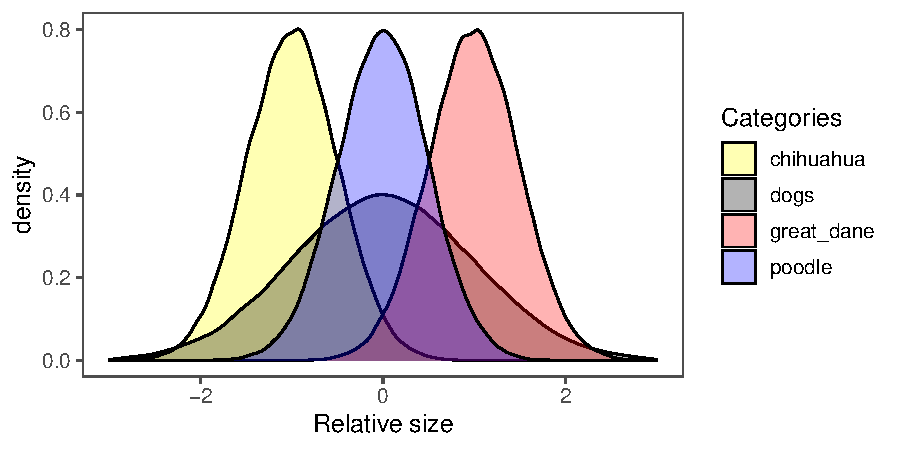
\includegraphics[width=0.7\linewidth]{refpred-RSA_priors.pdf}
	\end{center}
	\vspace{-0.3cm}
	\caption{Hypothetical prior size distributions over a basic-level, a small-subordinate, a medium-subordinate and a large-subordinate category. These distributions were used for qualitative tests of the refpred-RSA model.}
	\label{model1-priors}
\end{figure*}

Since the literal listener infers states consistent with the literal meaning of utterances, the representation of literal semantics of the utterance she observes is a crucial component of the model. This model employs classic Boolean semantics common in RSA models \parencite{montague1973proper, problang}. For the meaning computation, the utterance is split into subject and predicate, and each component is evaluated with respect to one goal (reference or predication, respectively); an utterance is assumed to be true of a state if and only if both components are true.  When computing the meaning of the subject, the bare deictic `that' and the basic-level nouns are assumed to be true of any member of the context, while subordinate labels only apply to respective category members. The referential utility of the subject is therefore formalized as in the vanilla RSA model (s.~Section~\ref{intro-rsa}). The meaning of the predicate is computed in terms of threshold semantics, as first proposed by \textcite{lassiter2013context}: 
\begin{equation}
\llbracket u \rrbracket (s, r) = \llbracket u_{Subj} \rrbracket (r) \land \llbracket u_{Pred} \rrbracket_{\theta} (s) = \llbracket u_{Subj} \rrbracket (r) \land \theta > s
\end{equation}
%\pt{Predictions of the different models / conceptual differences / discussion and comparison to E3; potentially move a part to Appendix}
  
So putting all these elements together, the proposed model formalizes a pragmatic listener inferring an intended referent in context, its size and the intended comparison class upon observing a sentence containing a noun and an adjective:
\begin{gather*}
	L_1 (r, s, cc \mid u, C) \propto P_{S_1} (u, cc \mid s, r, C) \; P(r, s \mid C, cc_{r\_sub}) \\
	S_1 (u, cc \mid s, r, C)  \propto exp(\alpha \: log \: L_0 (s, r \mid u, C, cc) \; P(cc) \; P(u)) \\
	L_0 (r, s \mid u, cc, C) \propto \llbracket u_{Subj} \rrbracket (r)  \;  \llbracket u_{Pred} \rrbracket^{\theta} (s) \; P(r, s \mid C, cc) \; P(\theta)
\end{gather*}
 
\begin{figure*}[t]
 	\begin{center}
 		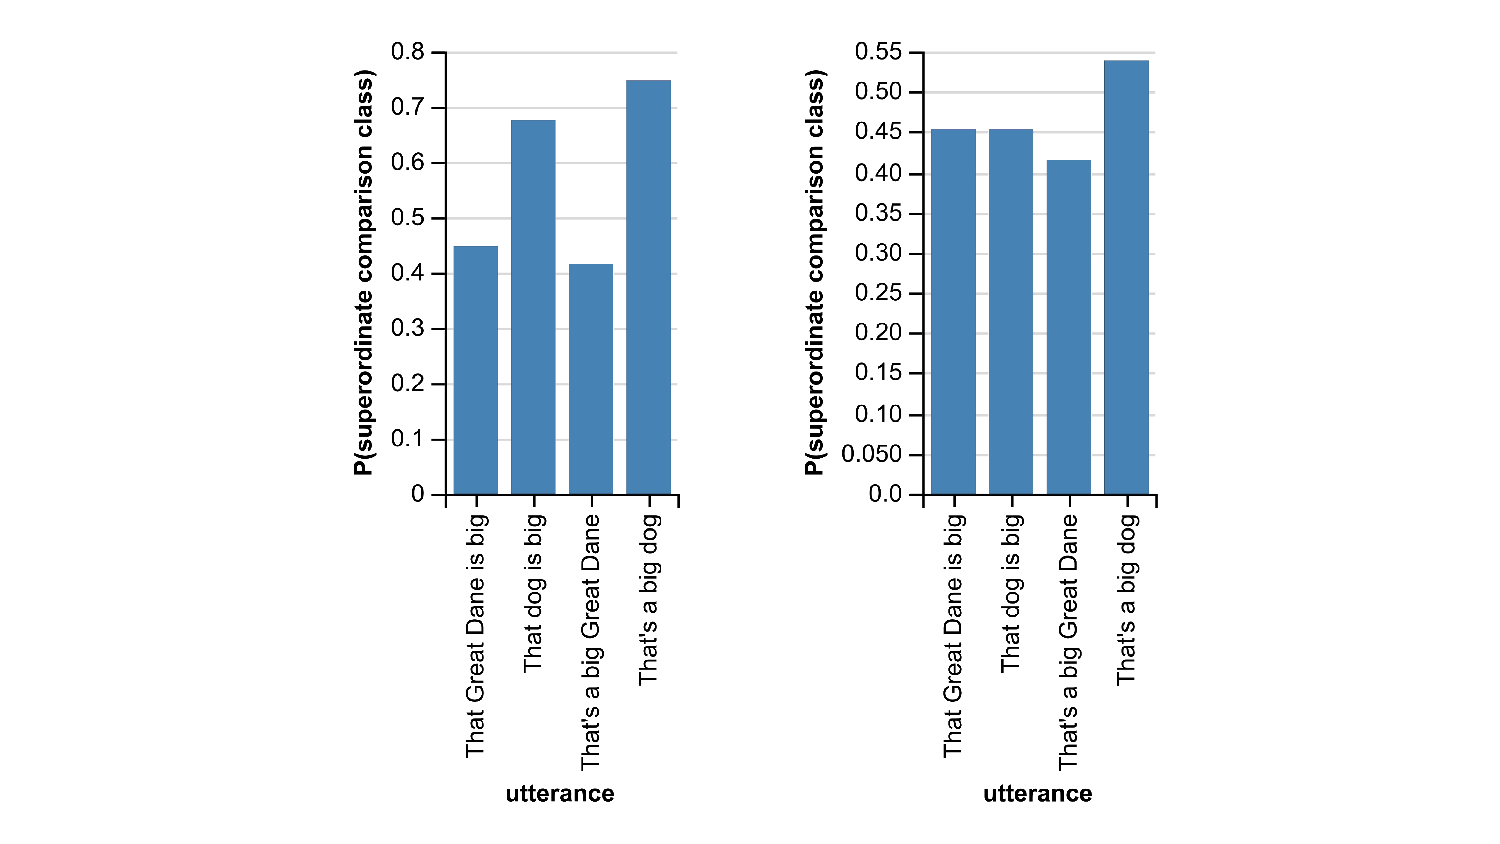
\includegraphics[width=\linewidth]{model1-cc-posteriors.pdf}
 	\end{center}
 	\vspace{-0.3cm}
 	\caption{Qualitative predictions made by the refpred-RSA model: Pragmatic listener inferences are plotted in terms of the probability to use the basic-level comparison class (i.e., ``big for a dog"), given utterances differing in the noun and its position, presented in a basic-level context (left)~vs.~subordinate context (right). Qualitatively, the crucial noun$\times$syntax interaction can be observed. Note the different y-axis scaling.}
 	\label{model1-cc-results}
 \end{figure*}
In order to investigate whether the qualitative predictions of this model capture the essence of predictions made by the reference-predication hypothesis, supported by the data observed in Experiment 3, the model was implemented using the probabilistic programming language WebPPL \parencite{dippl}. The pragmatic listener model was then tested on example sentences matching critical conditions from Experiment 3 (s. Section \ref{experiment3}). Most importantly, the model should capture the contrast in comparison classes inferred from subordinate-noun sentences differing in the position of the noun, distinct from basic-level noun sentences.

Figure \ref{model1-cc-results} (left) shows the proportion of basic-level comparison classes (i.e., ``big for a dog") the model predicts upon observing example utterances containing the nouns ``dog"~vs.~``Great Dane", appearing in the subject~vs.~predicate position, given a basic-level context. 
Visually, the critical contrasts can be observed: the model predicts that the basic-level comparison class is less likely given the utterance ``That's a big Great Dane", relative to ``That Great Dane is big". Furthermore, the model captures that the basic-level comparison class is generally less likely if the utterance contains a subordinate noun. Finally, the pragmatic listener infers more basic-level comparison classes given the utterance ``That's a big dog" than the utterance ``That dog is big", which is generally consistent with reference-predication hypothesis predictions, though was not observed in Experiment 3 due to a ceiling effect in the basic-level context (s. Figure \ref{cci-results}). 

\begin{figure*}[t]
	\begin{center}
		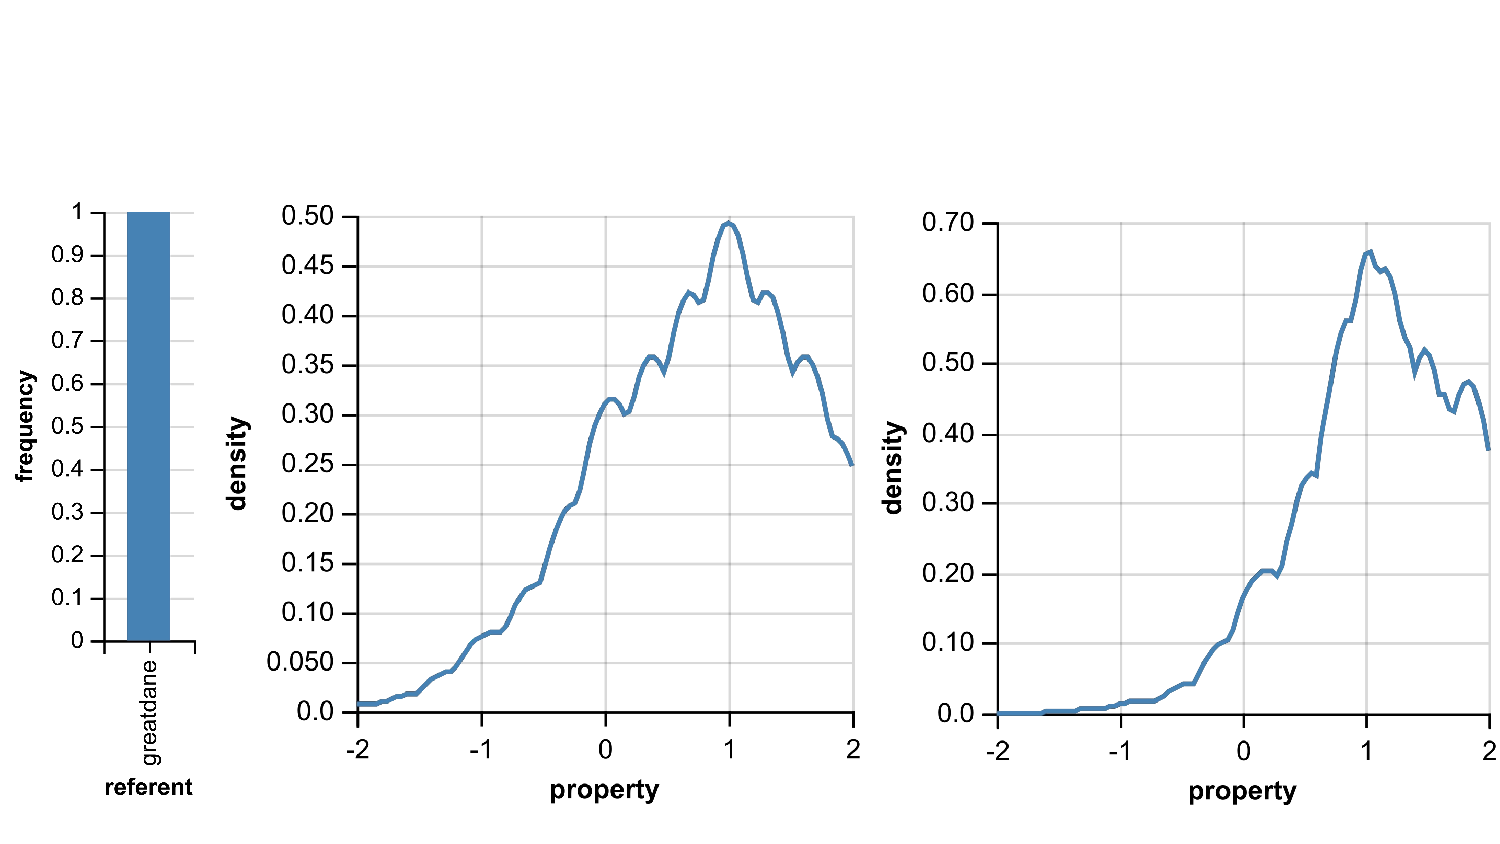
\includegraphics[width=\linewidth]{model1-ref-size-posteriors.pdf}
	\end{center}
	\vspace{-0.3cm}
	\caption{Qualitative predictions made by the refpred-RSA model: Given the utterance ``That Great Dane is big", the pragmatic listener infers a large-subordinate size distribution (middle) and is certain that the referent is a Great Dane (left). Given the utterance ``That's a big Great Dane", the pragmatic listener shifts her size distribution even more towards large size values (right), and is again certain about the referent (left).}
	\label{model1-ref-size-results}
\end{figure*}
\begin{figure*}[h]
	\begin{center}
		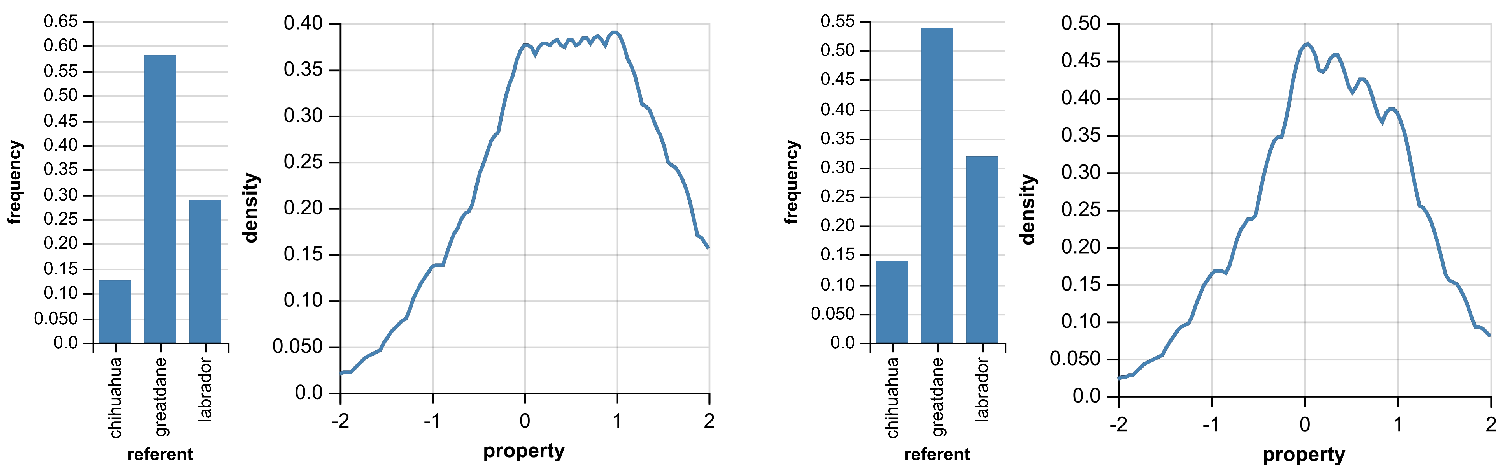
\includegraphics[width=\linewidth]{model1-basicN-basicC-crop.pdf}
	\end{center}
	\vspace{-0.3cm}
	\caption{Qualitative predictions made by the refpred-RSA model given the utterances with a basic level noun in basic-level context (from left to right): distribution over referents, distribution over sizes inferred from ``That dog is big" (subject N); distribution over referents, distribution over sizes inferred from ``That's a big dog".}
	\label{model1-basicN-basicC}
\end{figure*}
\begin{figure*}[b]
	\begin{center}
		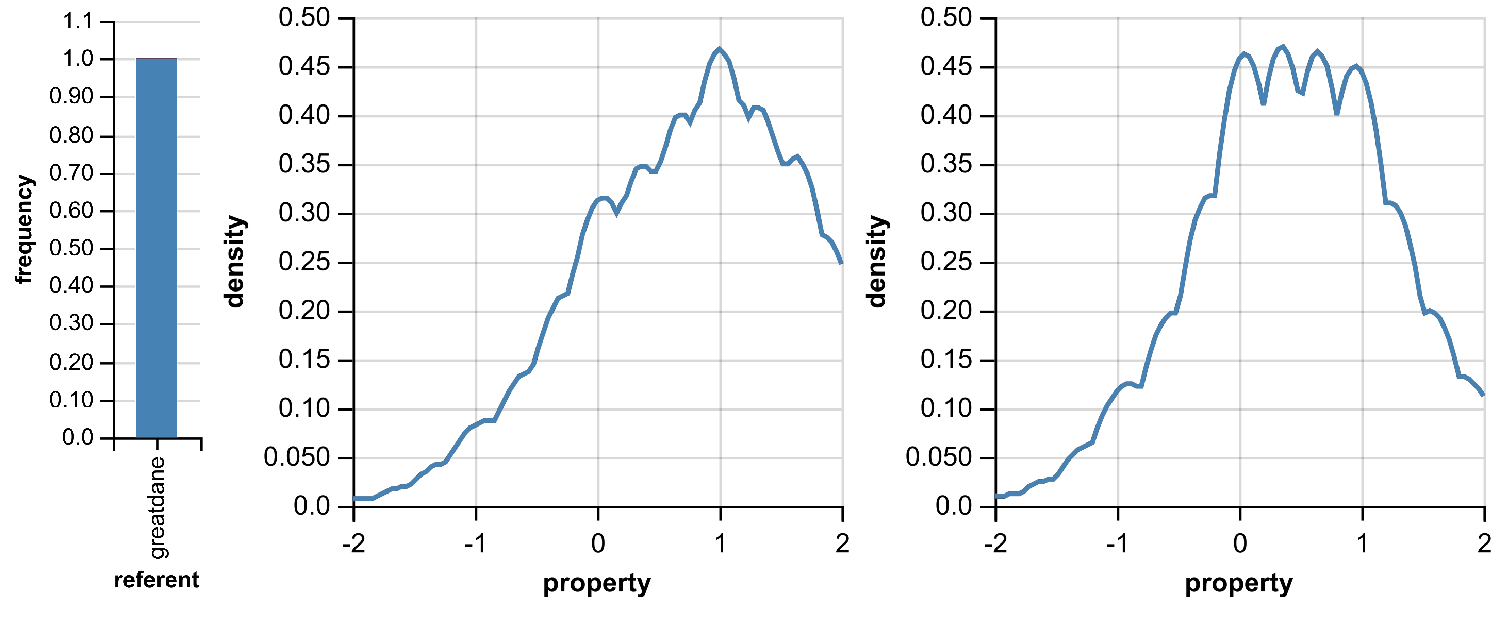
\includegraphics[width=\linewidth]{model1-basicN-subC-crop.pdf}
	\end{center}
	\vspace{-0.3cm}
	\caption{Qualitative predictions made by the refpred-RSA model given the utterances with a basic level noun in subordinate context (from left to right): distribution over referents, distribution over sizes inferred from ``That dog is big" (subject N); distribution over sizes inferred from ``That's a big dog".}
	\label{model1-basicN-subC}
\end{figure*}

The model performs comparably well given the same utterances in \emph{subordinate} context (Fig.~\ref{model1-cc-results}, right). First, consistent with data observed in Experiment 3, the model captures a grand influence of context: overall, the basic-level comparison class is less likely given the subordinate context than the basic-level context (Fig.~\ref{model1-cc-results}, left~vs.~right). Second, the model captures reasoning about contextual referential utility, rendering both nouns in the subject position equally referentially uninformative. Finally, both nouns in the predicate position are more likely to signal their respective comparison class than in the subject position.

In both contexts, given the critical utterances containing a subordinate noun, the model infers the expected referent and size distributions (Fig.~\ref{model1-ref-size-results}). That is, the inferred referent matches the noun; the inferred size distribution is shifted more strongly towards the subordinate category size values when observing an utterance containing a predicate noun relative to an utterance containing a subject noun. 
When the noun is the basic-level target label, in the basic-level context the pragamtic listener is uncertain about the intended category of the referent (Fig.~\ref{model1-basicN-basicC}). As predicted, the inferred size distributions do not differ qualitatively in the basic-level context across the two sentence frames, but do so in subordinate context: when the noun appears in the predicate, the listener shifts her distribution more towards the basic-level category properties, but infers a more subordinate --- i.e., contextually informed --- distribution when the noun is in the subject (Fig.~\ref{model1-basicN-subC}). These results provide further support that the model represents the reference-predication hypothesis well.

In sum, this model formalizes the reference-predication trade-off hypothesis via recursive probabilistic reasoning, representing the pragmatic listener as considering an agent enriching the adjective meaning to convey a particular comparison class. It integrates reasoning about both syntactic and semantic aspects of the utterance and generally captures comparison class inferences observed empirically, driven by the trade-off of the noun utility for different informational goals. It was shown that such a complex inferential hypothesis can be qualitatively explained by minimally extending existing generic Rational Speech Act tools. To the best of our knowledge, this is the first attempt to formalize reasoning about both meaning and structure of an utterance within the RSA framework,  contributing to both creating more accurate gradable adjective interpretation models and extending the scope of RSA models. 
